\section{Results}
The raw dataset was already divided into a training set and a testing set. We subjected it to text preprocessing and applied tokenization.

\begin{figure*}[ht]
\centering
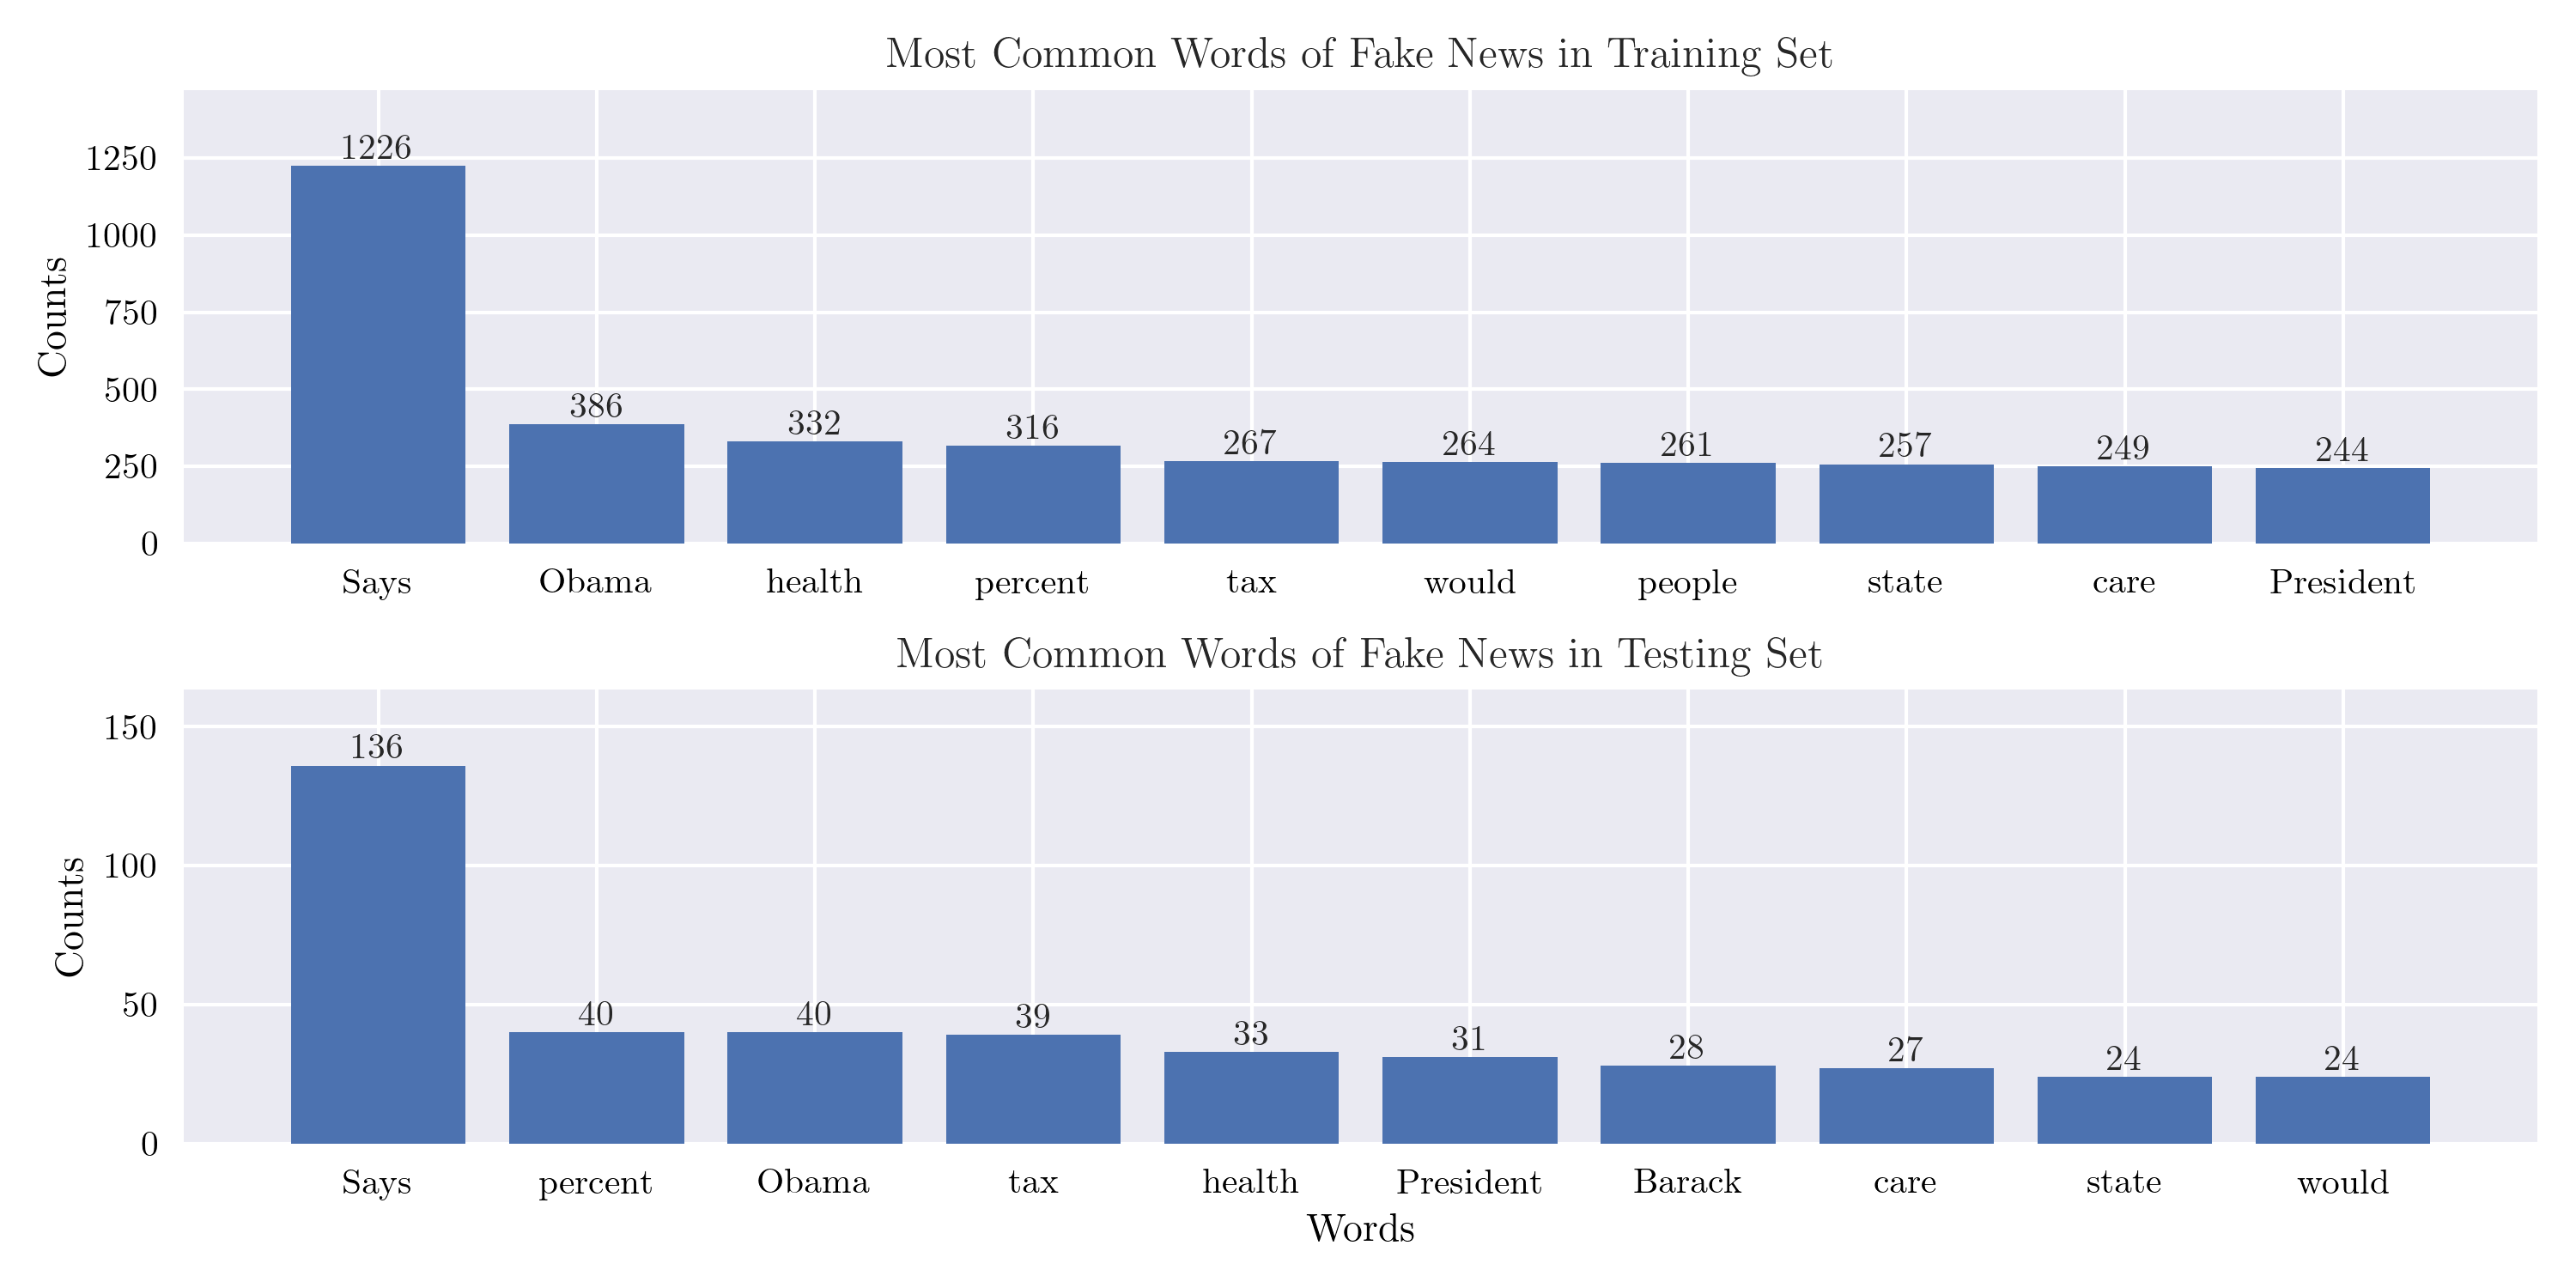
\includegraphics[width=0.95\linewidth]{top10_common_words_fake.png}
\caption{Top 10 most common words for fake news}
\label{top10_common_words_fake}
\end{figure*}

\

\begin{figure*}[ht]
\centering
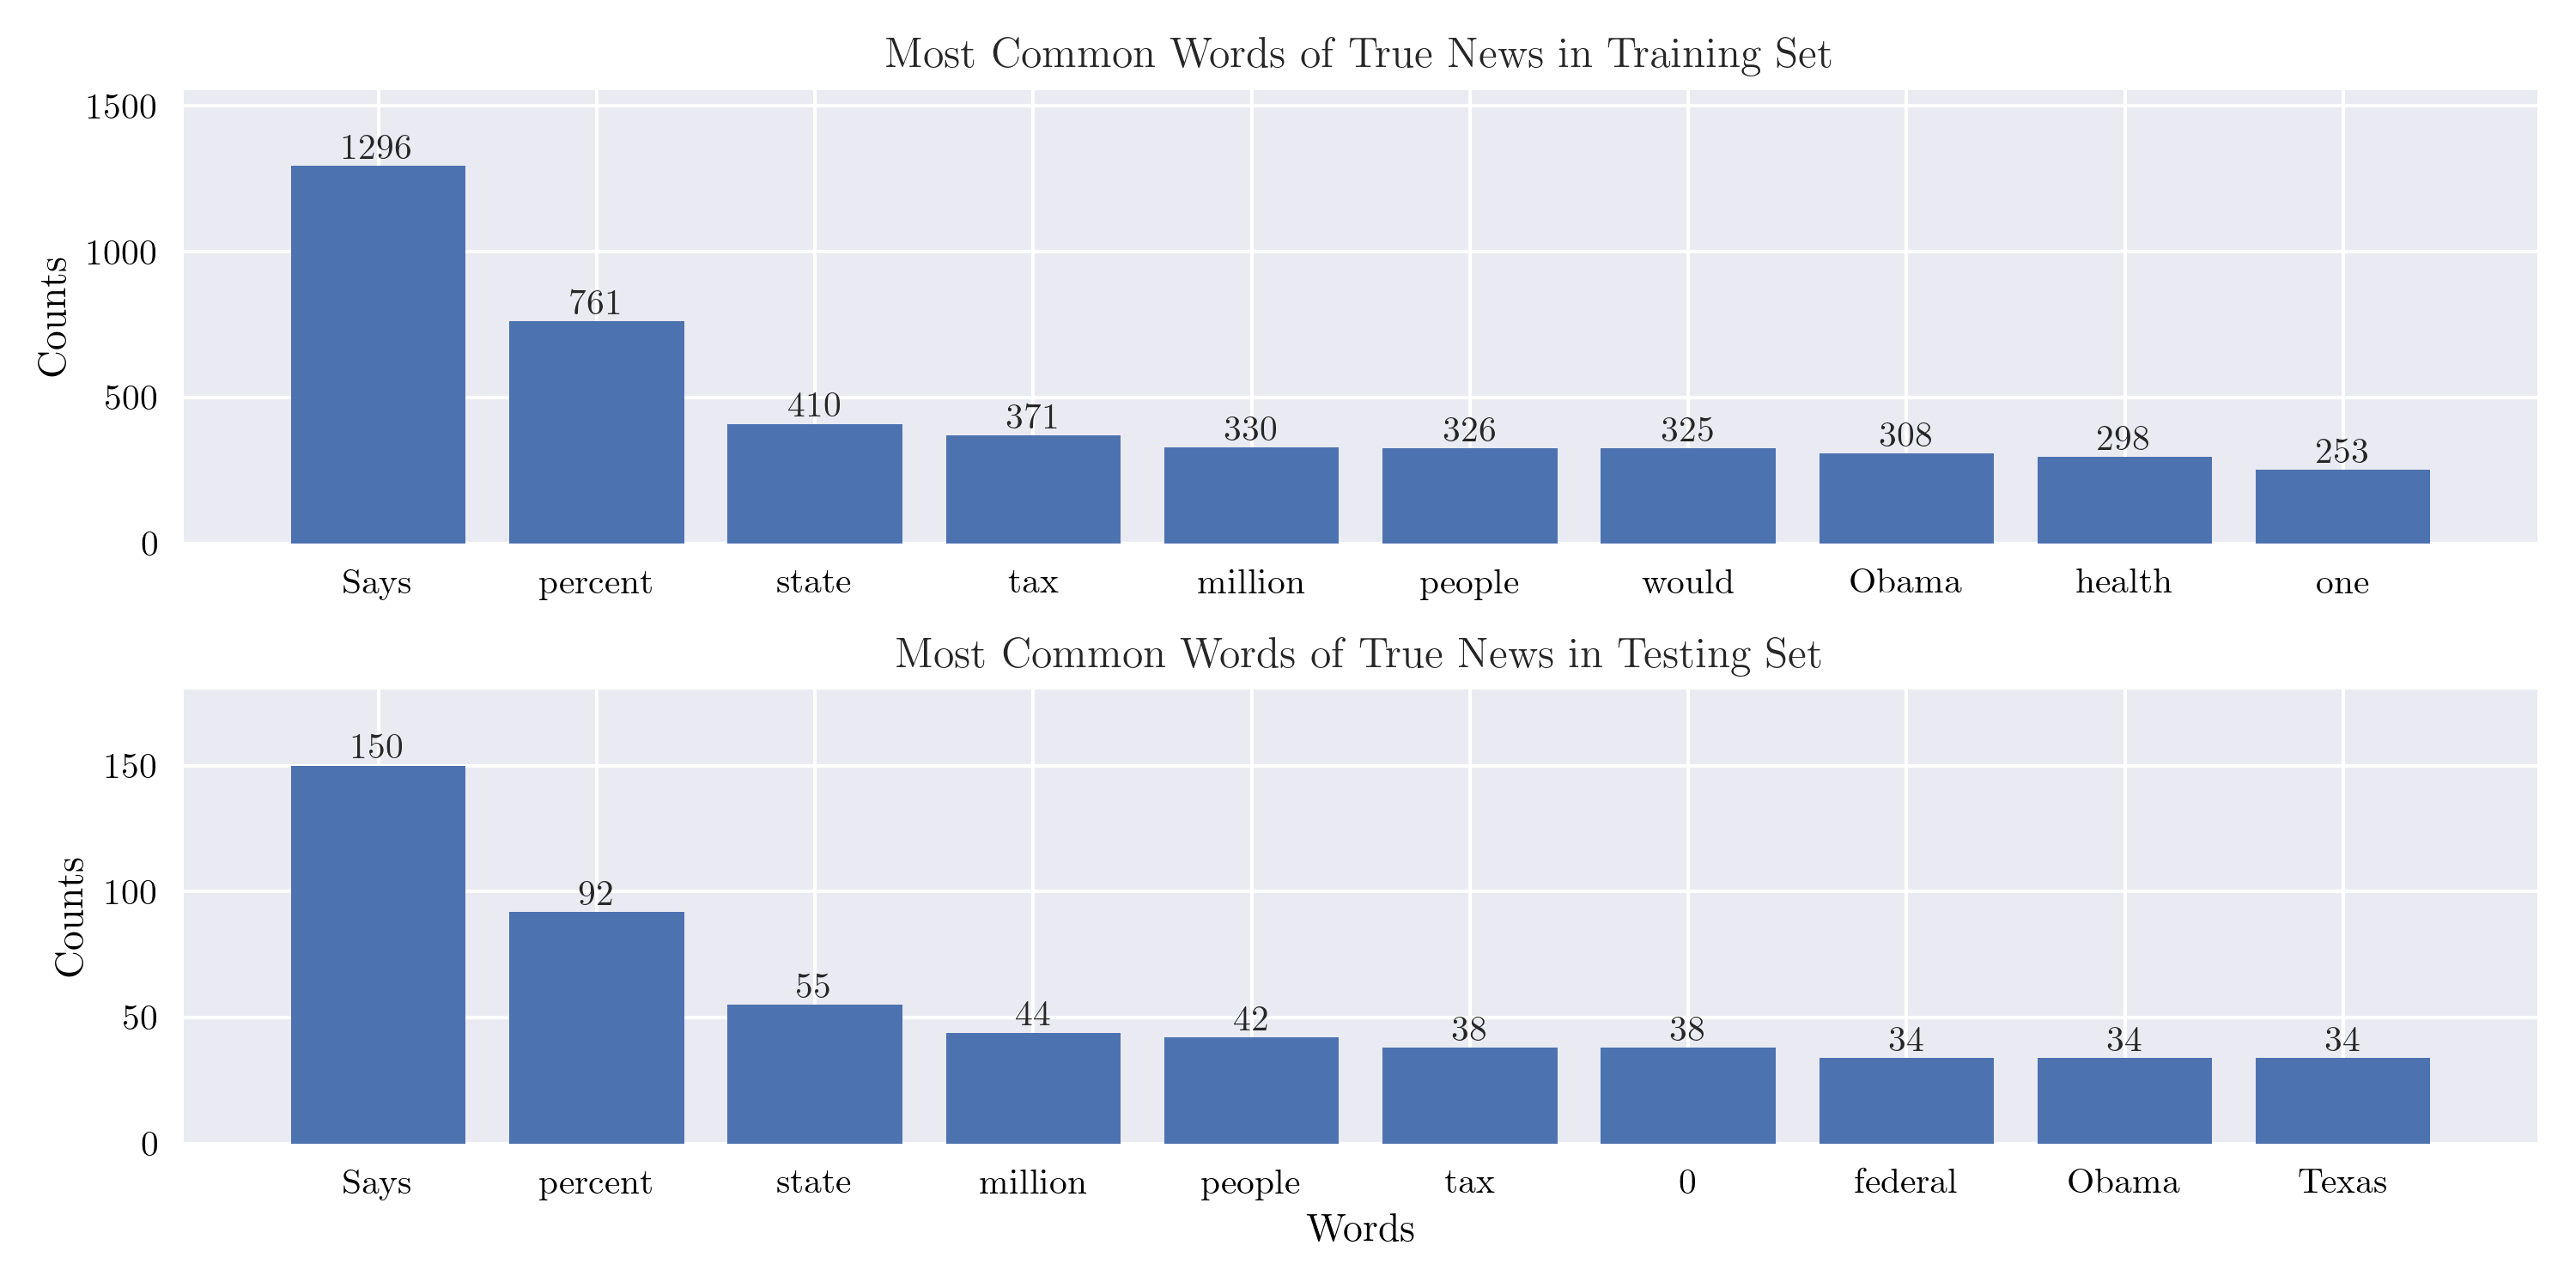
\includegraphics[width=0.95\linewidth]{top10_common_words_true.png}
\caption{Top 10 most common words for true news}
\label{top10_common_words_true}
\end{figure*}

The prepared dataset was examined with regard to the most common words. The analysis was divided based on the training and testing sets, as well as the type of news, whether it is a fake news (Figure~\ref{top10_common_words_fake}) or true news (Figure~\ref{top10_common_words_true}). The analysis of the following charts allows us to conclude that no distinct pattern of the most popular words stands out among the identified groups, which could disrupt the study.

Using the architecture described in the previous section, we built separate models for each combination of embedding and classification algorithms. To verify the research hypotheses, it was necessary to examine the performance of each model thoroughly.

Since the study operated on a slightly imbalanced dataset, closer attention had to be paid to the issue of selecting appropriate metrics. Not all metrics are suitable for use on imbalanced data. In this case, an example of an incorrect metric would be accuracy. Accuracy is calculated as the ratio of correctly classified samples to the total number of samples, regardless of the class distribution. Therefore, when one class predominates numerically over the other, the model can achieve high accuracy simply by assigning all predictions to the majority class, thus making poor predictions on the less numerous class.

In the case of imbalanced data, a much better choice would be to use metrics such as Balanced Accuracy, F1 Score, or AUC-ROC, which were employed in this study.

Balanced Accuracy is a metric that deals with imbalanced classes by introducing a balanced evaluation of the model's performance on each class. It is the average percentage of true positive results that have been correctly classified (in other words, recall or sensitivity) for each class. However, Balanced Accuracy does not take into account precision, which focuses on the ratio of correct positive classifications. Depending on the goal we want to achieve when building a model, we may be interested in different metrics. For example, precision is crucial when the priority is to minimize false positives.


\begin{table}[htb]
\centering
\begin{tabular}{l|c|c|c|c|c}
\hline

% OLD
%\multicolumn{2}{c|}{\multirow{2}{*}{Model}} & \multicolumn{2}{c}{Score} \\
%\cline{3-4}
%\multicolumn{1}{l}{} & & Accuracy & F1-Score\\

% NEW
\multicolumn{2}{c|}{Model} & \multicolumn{4}{c}{Score} \\
\cline{1-6}
Embedding & Classification & Accuracy & B. Accuracy & F1 Score & ROC AUC \\

\hline
\multirow{6}{*}{GloVe}
    & Logistic Regression & 60.1 & 58.4 & 49.3 & 58.4 \\
    & KNN & 55.3 & 53.9 & 45.5 & 53.9 \\
    & SVM Classifier & 59.2 & 57.9 & 50.3 & 57.9 \\
    & Random Forest & 60.0 & 58.4 & 49.9 & 58.4 \\
    & XGBoost & 61.2 & 59.3 & 49.7 & 59.3 \\
    & Neural Network & 60.6 & 60.2 & \textbf{55.7} & 60.2 \\
\hline
\multirow{6}{*}{Word2Vec}
    & Logistic Regression & 61.7 & 59.7 & 49.9 & 59.7 \\
    & KNN & 54.0 & 53.4 & 47.9 & 53.4 \\
    & SVM Classifier & 60.5 & 59.4 & 53.0 & 59.4 \\
    & Random Forest & 57.9 & 56.1 & 46.6 & 56.1 \\
    & XGBoost & 57.1 & 56.0 & 48.7 & 56.0 \\
    & Neural Network & 60.6 & 59.9 & \textbf{54.6} & 59.9 \\
\hline
\multirow{6}{*}{BERT} 
    & Logistic Regression & 60.5 & 58.9 & 50.7 & 58.9 \\
    & KNN & 55.9 & 54.9 & 48.3 & 54.9 \\
    & SVM Classifier & 58.6 & 57.4 & 50.3 & 57.4 \\
    & Random Forest & 57.6 & 45.7 & 45.7 & 55.7 \\
    & XGBoost & 59.4 & 58.0 & 50.1 & 58.0 \\
    & Neural Network & 58.8  & 57.8 & \textbf{53.7} & 57.8 \\
\hline
\multirow{6}{*}{RoBERTa} 
    & Logistic Regression & 60.1 & 58.9 & 52.0 & 58.9 \\
    & KNN & 56.9 & 55.9 & 49.2 & 55.9 \\
    & SVM Classifier & 61.5 & 60.2 & 53.1 & 60.2 \\
    & Random Forest & 59.1 & 57.0 & 46.5 & 57.0 \\
    & XGBoost & 58.3 & 57.1 & 49.7 & 57.1 \\
    & Neural Network & 62.0 & 61.0 & \textbf{54.8} & 61.0 \\
\hline
\multirow{6}{*}{GPT-2} 
    & Logistic Regression & 62.0 & 60.6 & 53.6 & 60.6 \\
    & KNN & 55.2 & 53.4 & 43.4 & 53.4 \\
    & SVM Classifier & 61.6 & 60.1 & 52.2 & 60.1 \\
    & Random Forest & 58.8 & 57.0 & 47.8 & 57.0 \\
    & XGBoost &  60.1 & 58.6 & 50.6 & 58.6 \\
    & Neural Network & 60.3 & 59.7 & \textbf{54.6} & 59.7 \\
\hline
%\multicolumn{2}{c|}{Total Variables}     & 28,946 & 356 & 21,443 & 23,962\\
%\multicolumn{2}{c|}{Residual Error Mean} & 3.04   & 3.50 & 2.92  & 2.93 \\
%\hline
\end{tabular}
\caption{Performance metrics for all combinations of embeddings and classification algorithms on a test set}
\label{results_table}
\end{table}

Another metric that can be successfully used to measure the performance of a model on an imbalanced dataset is the F1 Score. The F1 Score is the harmonic mean of precision and recall. It introduces a balance between precision and recall, which is useful when we want to consider both false positives and false negatives. The F1 Score takes values in the range of 0 to 1, with values closer to 1 indicating a better model. This metric is useful when assigning equal weight to the consequences of false positives and false negatives. Since we are looking for a metric that best compares performance while disregarding the business aspects of the model (such as modifying cutoff points to achieve a specific outcome), we consider it an appropriate metric for comparing models in this study.

The Area Under the Receiver Operating Characteristic Curve (AUC-ROC) measures the performance of a classification model. The ROC curve is a graphical representation of the tradeoff between true positive rate and false positive rate for different cutoff points. Similar to the F1 Score, it takes values between 0 and 1, where 1 denotes a perfect model, and 0.5 denotes a model that is no better than random. It is worth noting, however, that the AUC-ROC result is an average value across all threshold levels. Since this study focuses only on the default threshold level of 0.5, we choose the F1 Score as the leading and decisive metric for selecting the best model.


Analyzing the results, we conclude that none of the models proved to be better than the best model presented by Khan et al. (55.7 vs. 62.0 F1 Score). However, the goal of this study was not to build the best-performing model but to compare how different tools affect the model's performance. When analyzing the embedding methods, it is difficult to determine if any of the methods turned out to be the best. To verify the hypothesis that language models outperform the other embedding methods used in this study, we employed the Kruskal-Wallis test. This test compares the distributions of a particular variable in multiple independent groups and determines whether the distributions do not differ between groups. This test is a non-parametric alternative to one-way ANOVA – does not assume data normality and can be used to compare groups of different sizes.

We employ the Kruskal-Wallis test to verify the initial research hypothesis by comparing the F1 Score results for each embedding method. In this manner, we compare 30 observations, with six in each of the five groups. The results of the test indicate that the performance of different embedding models does not differ significantly from each other. The p-value of the Kruskal-Wallis test was 0.98. Therefore, at any significance level there is no basis for rejecting the null hypothesis that the distribution of performance scores of individual embedding methods differ from each other.

% We employ the Friedman test to verify the initial research hypothesis by comparing the F1 Score results for each embedding method. In this manner, we compare 30 observations, with six in each of the five groups. The results of the test indicate that the performance of different embedding models does not differ significantly from each other. The p-value of the Friedman test was 0.53. Therefore, at any significance level there is no basis for rejecting the null hypothesis that the median performance scores of individual embedding methods differ from each other.

The research hypothesis that language models (BERT, RoBERTa, GPT-2) outperform the other embedding methods (Word2Vec, GloVe) was not confirmed.

To verify the second null hypothesis that some classification algorithms perform better than others, we conducted a similar test among different classification methods. We compare the performance, measured by F1 Score, of individual groups of classification methods, which differ from one another. Within each group, we test the F1 Score results for the same classification methods, but using different embedding methods. In total, we examine 30 observations, divided into six groups, each consisting of five instances.
The p-value of the Kruskal-Wallis test was <0.001 (=0.0002). Therefore, at any sensible significance level the null hypothesis that the distribution of performance scores of individual classification methods is the same has to be rejected.

The research hypothesis that the choice of classification algorithm significantly affects the model's results has been confirmed statistically.
However, the Kruskal-Wallis test does not indicate which of the examined groups differs from the others. To determine which group differs from the others, it would be necessary to perform pairwise comparisons between the groups. 

In order to achieve this, I perform a post-hoc test for the Kruskal-Wallis test -- the Dunn test. This test compares individual groups in pairs and returns p-values for each comparison of means. The Dunn test examines the null hypothesis of equal means. If the p-value is smaller than the significance level, there is evidence to reject the null hypothesis of the test and conclude that the means in the examined groups differ.

% In order to achieve this, I perform a post-hoc test for the Friedman test -- the Nemenyi test. This test compares individual groups in pairs and returns p-values for each comparison of means. The Nemenyi test examines the null hypothesis of equal means. If the p-value is smaller than the significance level, there is evidence to reject the null hypothesis of the test and conclude that the means in the examined groups differ.

\begin{table}[htb]
\centering
{
\makegapedcells
\begin{tabular}{l|llllll}
    & LR    & KNN            & SVM   & RF             & XGB   & NN             \\ \hline
LR  & 1.000 & 0.337          & 1.000 & 0.510          & 1.000 & 1.000          \\ 
KNN & 0.337 & 1.000          & 0.095 & 1.000          & 1.000 & \textbf{0.001} \\ 
SVM & 1.000 & 0.095          & 1.000 & 0.153          & 1.000 & 1.000          \\
RF  & 0.510 & 1.000          & 0.153 & 1.000          & 1.000 & \textbf{0.002} \\
XGB & 1.000 & 1.000          & 1.000 & 1.000          & 1.000 & 0.161          \\
NN  & 1.000 & \textbf{0.001} & 1.000 & \textbf{0.002} & 0.161 & 1.000  
\end{tabular}
}
\caption{Dunn post-hoc pairwise test results}
\label{dunn_pairwise}
\end{table}

% \begin{table}[htb]
% \centering
% {
% \makegapedcells
% \begin{tabular}{l|llllll}
%     & LR    & KNN            & SVM   & RF             & XGB   & NN             \\ \hline
% LR  & 1.000 & 0.326          & 0.900 & 0.430          & 0.900 & 0.533          \\ 
% KNN & 0.326 & 1.000          & 0.114 & 0.900          & 0.826 & \textbf{0.003} \\ 
% SVM & 0.900 & 0.114          & 1.000 & 0.168          & 0.728 & 0.826          \\
% RF  & 0.430 & 0.900          & 0.168 & 1.000          & 0.900 & \textbf{0.005} \\
% XGB & 0.900 & 0.826          & 0.728 & 0.900          & 1.000 & 0.114          \\
% NN  & 0.533 & \textbf{0.003} & 0.826 & \textbf{0.005} & 0.114 & 1.000  
% \end{tabular}
% }
% \caption{Nemenyi post-hoc pairwise test results}
% \label{nemenyi_pairwise}
% \end{table}

% Table~\ref{nemenyi_pairwise} presents the p-values of the Nemenyi test results for each comparison between classification methods. With a significance level of 0.05, there is evidence to reject the null hypothesis of equal means for two groups: Neural Network vs. KNN (p-value = 0.003) and Neural Network vs. Random Forest (p-value = 0.005). This implies that the classification results obtained using Neural Network statistically differ from those obtained using KNN and Random Forest. No significant differences between means were found for the remaining groups.

Although the Dunn test results did not indicate the superiority of Neural Network over all classification methods, they suggest that this classification method tends to dominate over the other classification methods.

Indeed, upon analyzing the results table (Table~\ref{results_table}), it can be observed that for each embedding method, considering the F1 Score, Neural Network turned out to be the best. The best overall model was the one with GloVe embeddings and Neural Network classification (F1 Score = 55.7).

%\begin{table}[htb]
%\centering
%{
%\makegapedcells
%\begin{tabular}{cc|cc}
%\multicolumn{2}{c}{}
%            &   \multicolumn{2}{c}{Predicted} \\
%    &       &   Yes &   No              \\ 
%    \cline{2-4}
%\multirow{2}{*}{\rotatebox[origin=c]{90}{Actual}}
%    & Yes   & 331   & 487                 \\
%    & No    & 165    & 284                \\ 
%    \cline{2-4}
%    \end{tabular}
% }
%\caption{Confussion matrix for the GPT-2+KNN model}
%\label{gpt2knn_cm}
%\end{table}

\begin{table}[htb]
\centering
{
\makegapedcells
\begin{tabular}{lll}
                & Predicted negative & Predicted positive \\
\hline
Actual negative & 454 (TN)           & 260 (FP) \\
Actual positive & 239 (FN)           & 314 (TP) \\
\hline
\end{tabular}
}
\caption{Confussion matrix for the GloVe + Neural Network model}
\label{glovenn_cm}
\end{table}

Upon analyzing the confusion matrix (Table~\ref{glovenn_cm}), it can be concluded that the best model successfully identified the majority of fake news and true news, exhibiting a relatively high number of true positives (TP) and true negatives (TN), while having a relatively low number of false positives (FP) and false negatives (FN).

